\section{\ldeen{Einführung}{Introduction}}
\subsection{\ldeen{Idee}{Idea}}
\ldeen{Lehrmaterialien treten in vielerlei Formen und Versionen auf, beispielsweise als
  Vorlesungsskript, Folien oder Handouts, und das möglicherweise jeweils in verschiedenen Sprachen.
  Dabei sind die Inhalte oft gleich oder ähnlich, und die Stukturen~-- beispielsweise die
  Reihenfolge der Lehr- und Lerneinheiten sollten konsistent sein.}{
  Teaching materials come in many forms and versions, such as
  lecture notes, slides, or handouts, and may be available in different languages.
  Yet the content is often the same or similar, and the structures—for example, the
  order of the teaching and learning units—should be consistent.
}
\ldeen*{Mit anderen Worten: Die gleiche Sache (hier: semantische Information) soll in unterschiedlicher Gestalt auftreten. In der Informatik oder in der Chemie nennt man dieses Konzept auch \emph{Polymorphie}@1.}{
  In other words: The same thing (here semantic information) should appear in different forms.
In computer science or chemistry, this concept is also known as \emph{polymorphism}@1
}{\footnote{\ldeen{
  Vielleicht wären \emph{Polyrepräsentation} oder sogar \emph{Multimodalität} noch passendere Begriffe,
  aber ersteres ist nicht sehr etabliert und beim zweiteren müsste ich vermutlich mit Kulturwissenschaftlern und Semiotikern darüber diskutieren, ob unterschiedliche Sprachen als \emph{Modi} aufzufassen sind.
  Außerdem bin ich Informatiker, da liegt die Polymorphie nahe.
  }{
    Perhaps \emph{poly-representation} or even \emph{multimodality} would be even more appropriate terms,
  but the former isn’t very well established, and with the latter, I’d probably have to discuss with cultural studies scholars and semioticians whether different languages should be understood as \emph{modes}.
  Besides, I’m a computer scientist, so polymorphism seems like a natural choice.}
}}

\ldeen{
  Gleichzeitig werden Lehrmaterialien in der Regel permanent überarbeitet. Einzelne Lehreinheiten
  werden modernisiert, reorganisiert oder gleich ganz entfernt, neue werden ergänzt.
}{
  At the same time, teaching materials are generally revised on an ongoing basis.
  Individual teaching units are updated, reorganized, or removed entirely, while new ones
  are added.
}
\ldeen*{
  Dabei stets die gewünschte Konsistenz aufrechtzuerhalten, ist schwierig. Das @1 Bundle
  versucht, Lehrende dabei zu unterstützen. Es folgt dabei einer zentralen Idee:
}{
  Maintaining the desired consistency throughout this process is difficult. The @1 Bundle
  aims to support instructors in this effort. It is based on a central idea:
}{\osglecture}
\footnote{
  \ldeen*{Es ist mir durchaus bewusst, dass dieser Leitgedanke nicht allgemein geteilt wird:
  ein \LaTeX-Riese wie \name{Joseph Wright} steht dieser Idee z.\,B. skeptisch gegenüber (@2),
  und er kann gute Gründe anbringen. Falls Sie also glauben, dass solche Gründe überwiegen, nutzen Sie @1 nicht.}{I am well aware that not everyone shares this guiding principle;
  a \LaTeX giant like \name{Joseph Wright}, for example, is skeptical of this idea (@2),
  and he can cite good reasons for his skepticism. So if you believe that such reasons outweigh the benefits, do not use @1.}
  {\osglecture}
  {\url{https://github.com/josephwright/ltx-talk/discussions/68\#discussioncomment-13755453}}
}
\begin{infobox}{\ldeen{Leitsatz}{Maxim}}\sffamily
\ldeen{Es sollten so \textbf{wenig} wie möglich \textbf{Redundanzen} auftreten.
  }{
    \textbf{Redundancies} should be kept to a \textbf{minimum}.
  }\medskip

  \ldeen{Wo Redundanzen notwendig sind (beispielsweise bei verschiedenen Textversionen),
  ist die Aufrechterhaltung von Konsistenz einfacher, wenn aufeinander
  bezogenes Quellmaterial \textbf{möglichst nahe} beieinander ist.
  }{
    Where redundancies are necessary (for example, with different versions of a text),
    it is easier to maintain consistency if related
    source material is located as \textbf{close together} as possible.}
\end{infobox}


\ldeen*{Daher soll @1 u.\,a.{} ermöglichen
}{
  Therefore, @1 is intended, amongst other things, to enable}{\osglecture}:
\begin{itemize}
  \item \ldeen{Generierung verschiedener Dokumentarten aus der gleichen Quelle
  }{
    Generating different types of documents from the same source
  };
  \item \ldeen{einfache Reorganisation von Lehreinheiten}{easy reorganization of teaching units};
  \item \ldeen{verschiedene Sprachvarianten aus der gleichen Quelle,
        wobei gemeinsame Daten nicht redundant dargestellt werden brauchen}{
        different language versions from the same source,
        wherein shared data does not need to be presented redundantly};
  \item \ldeen{Unterstützung bei individuellen Erstellen und Überarbeiten von
        Lehreinheiten mit einfacher Integration (z.\,B.{} Skriptkapitel zu einem
        Gesamtskript)}{
        support for creating and revising individual
        instructional units that can be easily integrated (e.g., lecture notes chapters into a
        comprehensive set of lecture notes)
        };
  \item \ldeen{schnelle Bereitstellung der verschiedenen Dokumentarten
  }{
    rapid deployment of the various types of document}.
\end{itemize}

\ldeen*{Dabei wurde von Modalitäten und Arbeitsabläufen ausgegangen, die
  an der Professur für Betriebssysteme (\emph{Operating Systems Group, OSG})
  der TU Chemnitz derzeit üblich sind.
  Wenn Sie nicht dort tätig sind und völlig andere Abläufe haben, könnte
  @1 trotzdem für Sie nützlich sein: einzelne Pakete des Bundles lassen sich
  auch unabhängig von den anderen nutzen.
  }{
    This was based on the procedures and workflows that
    are currently standard practice at the Operating Systems Group at Chemnitz University of Technology.
    If you do not work there and, for example, have different procedures,
    @1 might still be useful to you: individual packages within the bundle can
    also be used independently of the others.
  }{\osglecture}

\ldeen*{@1 ist das Nachfolgeprojekt von @2, das sich aus einem
  Thema und einer handvoll Ergänzungsmacros für die überaus verbreitete Beamer-Klasse@3
  entwickelt hat.
  Gegenüber seinem Vorgänger zeichnet sich @1 durch einen größeren Funktionsumfang,
  ein überarbeitetes und damit hoffentlich besseres Interface, eine umfangreichere
  Dokumentation und nicht zuletzt dadurch aus, dass es ermöglicht, barrierefreie getaggte
  Lehrdokumente zu erstellen, indem es Klassen wie \cls{ltx-talk} unterstützt.
  }{@1 is the successor project to @2, which has evolved from a
  theme and a handful of supplementary macros for the widely used Beamer class@3.
  }
  {\osglecture}
{\textcolor{teal!50!black}{OSG Beamer}\footnote{\url{https://github.com/tuc-osg/osgbeamer}}}
{\footnote{\url{https://ctan.org/pkg/beamer}}}

\subsection{\ldeen{Was genau \emph{ist} denn nun \osglecture?}{So what exactly \emph{is} \osglecture?}}
\ldeen{\osglecture{} ist ein \LaTeX-Bundle (genauer gesagt: ein \LuaLaTeX-Bundle), das verschiedene Ideen und Ansätze zusammenbringt um Lehrmaterialien zu erstellen. Keine dieser Ideen oder Ansätze ist besonders neu.
}{\osglecture{} is a \LaTeX bundle (more specifically, a \LuaLaTeX bundle) that brings together various ideas and approaches for creating teaching materials. None of these ideas or approaches is particularly new.}

\begin{itemize}
  \item \ldeen{
    \cls{osglecture} ist eine Metaklasse, die die meiste Arbeit an andere Klassen deligiert, so wie es z.\,B.{} auch \needpackage{beamerswitch} macht. Darüber hinaus stellt \cls{osglecture} aber
    auch einige Dinge selbst bereit, wie ein dokumentübergreifenden Referenzsystem und sogar einige 
    Fromatierungsumgebungen.
  }{
    \cls{osglecture} is a metaclass that delegates most of the work to other classes, much like 
    \needpackage{beamerswitch}, for example. In addition, \cls{osglecture} itself provides several features,
    including a cross-document reference system and even some formatting environments.}
  \item \ldeen{
    \pkg{langselect} ist ein Paket, das zur (sprachabhängigen) Auswahl von in das Ziel-PDF zu übernehmenden
    Text, ähnlich wie es auch \needpackage{comment} oder \needpackage{multilang} macht. 
    Die tatsächliche genutzte Sprache kann auch von außen festgelegt werden.
  }{
    \pkg{langselect} is a package for selecting which text is to be included in the target PDF depending on the 
    language, similar to \needpackage{comment} or \needpackage{multilang}. The language actually used can also 
    be specified externally.}
  \item \ldeen{
    \pkg{osglecture-modes} generalisiert die Idee von Darstellungsmodi, wie man sie aus \needpackage{beamer} 
    oder \needpackage{ltx-talk} kennt, macht also etwas ähnliches wie \pkg{langselect}, aber nicht auf
    Sprach- sondern auf Strukturebene. Damit können Modi in der aus \pkg{Peamer} oder \pkg{ltx-talk} 
    gewohnten \texttt{<>}-Syntay auch außerhalb von Präsentationen genutzt werden.
  }{
    \pkg{osglecture-modes} generalizes the concept of presentation modes familiar from \needpackage{beamer} 
    or \needpackage{ltx-talk}. It therefore does something similar to \pkg{langselect}, but at the structural 
    rather than the language level. This makes it possible to use modes outside presentations, too, with the 
    familiar \texttt{<>} syntax of \pkg{beamer} or \pkg{ltx-talk}.}
  \item \ldeen{
    \pkg{tagpax} dient dazu, getaggte PDF-Dokumente zu einem wiederum getaggten PDF-Dokument zu vereinen. 
    Es hat lange nicht soviel Möglichkeiten wie \needpackage{pdfpages} und baut auf den Ideen von 
    \needpackage{pax}/\needpackage{newpax} auf, behält aber nicht nur Annotationen sondern auch die 
    Taggingstruktur bei. Im Kontext von \osglecture{} dient es dazu, unabhängige Übersetzungen 
    z.\,B.\ einzelner Skriptkapitel zu einem Gesamtskript zu ermöglichen, ohne einen "`großen"' 
    Übersetzungslauf\footnote{Bei meinem Lehrskripten kann so ein großer Lauf durchaus auch mal über 
    eine Stunde dauern.} durchführen zu müssen.
  }{
    \pkg{tagpax} combines tagged PDF documents into a PDF document that is itself tagged. It provides far
    fewer features than \needpackage{pdfpages} and builds on the ideas of \needpackage{pax}/\needpackage{newpax}, 
    but preserves not only annotations, but also the tagging structure. In the context of \osglecture{}, it makes 
    it possible to compile, for example, individual lecture notes chapters independently and combine them into 
    a complete set of lecture notes without having to perform one "`large"' compilation run.\footnote{For my lecture
    notes, such a large run can sometimes take more than an hour.}
    }
  \item \ldeen{
    \OLLM{} ist ein \emph{yet another} Build-Tool, aber speziell auf \osglecture{} zugeschnitten und
    arbeitet eng mit \cls{osglecture} und den anderen genannten Paketen zusammen. Intern ruft \OLLM{} intern 
    \File{latexmk} auf (es ist aus einem rc-File für \File{latexmk} entstanden), das die meiste Arbeit erledigt.
  }{
    The \OLLM{} is a yet another build tool that is tailored specifically to \osglecture{} and works closely with 
    \cls{osglecture} and the other packages mentioned above. Internally, \OLLM{} invokes \File{latexmk}--it
    originated as an rc file for \File{latexmk}--which performs most of the work.}
\end{itemize}

\ldeen{Während diese genannten Pakete den Kern des Bundles bilden, gibt es noch einige Pakete, die sich 
  für die Erstellung von Lehrmaterialien als nützlich erwiesen haben. Diese interagieren durchaus mit den 
  Kernpaketen, tragen aber mehr zur direkten Gestaltung der Dokumente bei, als zur Realisierung des 
  Polymorphieansatzes, den sie aber nutzen.
}{While the packages mentioned above form the core of the bundle, several additional packages have proved 
  useful for creating teaching materials. They do interact with the core packages, but contribute more directly
  to the design of the documents than to implementing the polymorphism approach, although they make use of it.}
\begin{itemize}
  \item \ldeen{\pkg{osgstyler} versucht die \LaTeX-Kernidee der Trennung von Inhalt und Gestaltung
    über eine zentrale semantische Konfiguration zu stärken. Dinge wie Farben, Schriften, Abstände, Hervorhebungen
    und Blöcke können damit einerseits einfacher konsistent und andererseits leichter austauschbar gestaltet werden.
    Es kann gut mit \pkg{osglecture-modes} zusammenwirken.
  }{\pkg{osgstyler} seeks to reinforce the core \LaTeX{} principle of separating content from presentation 
    through a central semantic configuration. This makes elements such as colors, fonts, spacing, highlighting, 
    and blocks easier to design consistently as well as easier to replace. It works well in conjunction with \pkg{osglecture-modes}.}
  \item \ldeen{\pkg{ltxtalk-theme} ist eine experimentelle Theme-Engine für \cls{ltx-talk}. Für "`innere"'
    Gestaltungsaspekte wird \pkg{osgstyler} genutzt. Vermutlich wird \pkg{ltxtalk-theme} mit der weiteren Entwicklung
    von \cls{ltx-talk} irgendwann überflüssig.}{\pkg{ltxtalk-theme} is an experimental theme engine for 
    \cls{ltx-talk}. It uses \pkg{osgstyler} for inner design aspects. As \cls{ltx-talk} continues to evolve, 
    \pkg{ltxtalk-theme} will probably become obsolete eventually.}
  \item \ldeen{\pkg{lttheme-tuc-2019} ist die (inoffizielle) Umsetzung des offiziellen Präsentationslayout meiner
    Universität für \pkg{ltx-talk}. Es nutzt \pkg{ltxtalk-theme}.
  }{\pkg{lttheme-tuc-2019} is the unofficial implementation of my university's official presentation layout 
    for \pkg{ltx-talk}. It uses \pkg{ltxtalk-theme}.}
  \item \ldeen{\pkg{semcat} dient zur einfacheren semantischen Markierung (z.\,B.\ von Kategorien wie
    "`Hintergründe"',  "`technische Details"' oder "`Wiederholung"') von Textteilen oder QR-Codes.
  }{\pkg{semcat} facilitates the semantic labeling of passages of text or QR codes, for example with categories 
    such as "`background"', "`technical details"', or "`review"'.}
  \item \ldeen{\pkg{ansiterm} stellt zwei semiverbatim Umgebungen für die Darstellung von Computerterminalfenstern zur
    Verfügung, die ANSI-Escapesequenz\footnote{Siehe z.\,B.\ \url{https://de.wikipedia.org/wiki/ANSI-Escapesequenz}}
    interpretieren können. Eine davon führt zur Übersetzungszeit den Inhalt in einer Shell aus und liest die
    Ergebnisse zurück, simuliert also ein "`echtes"' Terminal.
  }{\pkg{ansiterm} provides two semiverbatim environments for displaying computer terminal windows that can 
    interpret ANSI escape sequences\footnote{See, for example, \url{https://en.wikipedia.org/wiki/ANSI_escape_code}.}. 
    One of them executes its contents in a shell at compilation time and reads back the results, thus simulating a 
    "`real"' terminal.}
  \item \ldeen{\pkg{osglistings} stellt ein Frontend für \needpackage{minted} zur Verfügung mit erweiterten 
    Möglichkeiten der Quellcodemarkierung, Einbindung von Gists und Repositories und verschiedenen Darstellungen.
  }{\pkg{osglistings} provides a front end for \needpackage{minted}, offering advanced source-code highlighting, the 
    inclusion of gists and repositories, and various presentation styles.}
\end{itemize}

\subsection{\ldeen{Polymorphie}{Polymorphism} in \osglecture}
\ldeen{Es ist eine alte \hologo{TeX}-Idee, Texte je nach Kontext unterschiedlich darzustellen. Die \hologo{TeX}-Variante \hologo{ConTeXt} leitet beispielsweise ihren Namen auch davon ab.
\osglecture{} versucht die Anwendung dieses Konzept noch ein Stück weit zu erweitern.
Dazu ist \cls{osglecture} eine \emph{Metaklasse}: Sie sagt (anders als die meisten
\LaTeX-Klassen) nicht, wie die fertig gesetzten Dokumente aussehen sollen,\footnote{Es gibt aber
Pakete im \osglecture-Bundle, die so etwas machen} sondern stellt ein gemeinsames Interfache zur
Verfügung und verteilt dann die Arbeit an Klassen wie \cls{article}, \cls{scrarticle}, \cls{beamer}
oder \cls{ltx-talk}.}{It is a
long-standing \hologo{TeX} concept to render text differently depending on the
context. The \hologo{TeX} variant \hologo{ConTeXt}, for example, derives its
name from this concept. \osglecture{} attempts to expand the application of this concept a bit further.
In this regard, \cls{osglecture} is a \emph{metaclass}: Unlike most
\LaTeX{} classes, it does not specify how the final typeset documents should look,\footnote{However, there are
packages in the \osglecture bundle that do just that} but rather provides a common interface
and then delegates the work to classes such as \cls{article}, \cls{scrarticle}, \cls{beamer},
or \cls{ltx-talk}.}

\ldeen{Das Folgende ist ein Mini-Showcase der zeigen soll, wie aus einer Quelle verschiedene Instanzen
erzeugt werden. Es dient lediglich dazu, dass der Nutzer einen kleinen Eindruck von den
Möglichkeiten des kontextabhängigen Polymorphismus in \osglecture{} gewinnen kann~-- die Diskussion
über Funktionsweise und die verwendeten Mechanismen erfolgt später.}{
The following is a mini-showcase designed to demonstrate how different instances are
created from a single source. Its sole purpose is to give the user a brief glimpse of the
possibilities of context-dependent polymorphism in \osglecture{}-—the discussion
of how it works and the mechanisms used will follow later.}

%\begin{figure}[h]
\begin{minipage}{\linewidth}
  \inputsourcecode[
    gobble=0,
    add-local-frame={innerleftmargin=12pt,innerrightmargin=8pt},
    add-sourcecode-options={breaklines=true,breakatwhitespace=true,
    columns=fullflexible,basicstyle=\footnotesize}
  ]{polymorphy-source.tex}
  \captionof{figure}{\label{fig:common-src}\ldeen{Gemeinsamer Quellcode}{Common source code}}
\end{minipage}

\begin{minipage}{\linewidth}
  \captionsetup{type=figure}
  \centering
  \begin{subcaptiongroup}
    \begin{minipage}[t]{.48\linewidth}
      \fbox{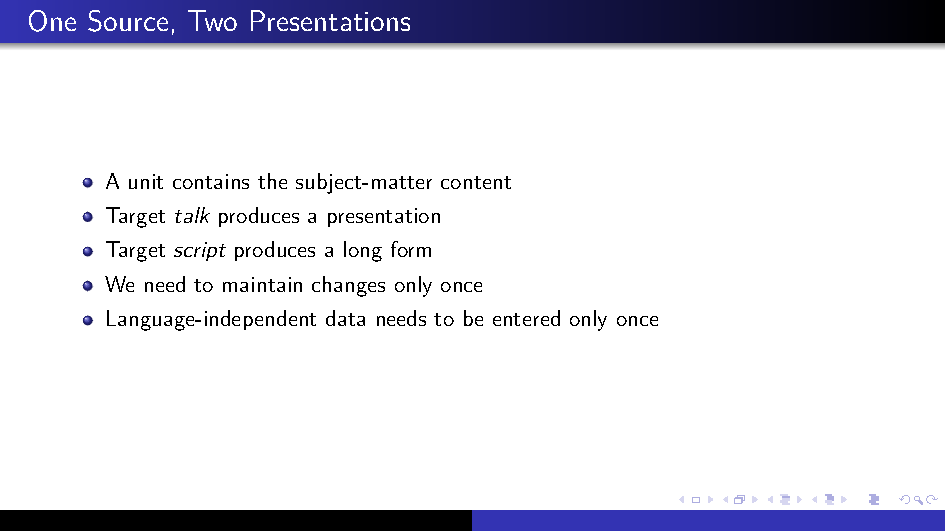
\includegraphics[page=1,width=\linewidth]{polymorphy-slides-en.pdf}}
      \caption{\ldeen{Folien auf English}{Slides in English}}
    \end{minipage}\hfill
    \begin{minipage}[t]{.48\linewidth}
      \fbox{\includegraphics[page=1,width=\linewidth]{polymorphy-slides-de.pdf}}
      \caption{\ldeen{Folien auf Deutsch}{Slides in German}}
    \end{minipage}

    \begin{minipage}[t]{.8\linewidth}
      \fbox{\includegraphics[page=1,width=\linewidth,
        trim=0mm 210mm 45mm 30mm,clip
      ]{polymorphy-script-de.pdf}}
    \caption{\ldeen*{Ausgabe für @1-Taget}{Version for @1-Taget}{\code{script}}}
    \end{minipage}
  \end{subcaptiongroup}
  \caption{\ldeen*{Alle Varianten sind aus der Quelle in Abb.~@4 erstellt:
    Bei den Folien in unterschiedlichen Sprachen @1 und @2 bleibt
    Gliederung, Aussagenfolge und Hervorhebung jeweils gleich, die Ausgabe für das Skript @3 ist inhaltlich äquivalent, jedoch  ausführlicher und in Satzform}%
  {All variants were created from the source shown in Fig.~@4:
    For the slides in different languages @1 and @2,
    the structure, sequence of statements, and emphasis remain the same in each case; the output for the script @3 is equivalent in content but  more detailed and in sentence form.}
  {(a)}{(b)}{(c)}
  {\ref{fig:common-src}}}
\end{minipage}
\medskip

\ldeen{Dass auch gewöhnlich Textauszeichnungen unterschiedlich gestaltet und damit polymorph sein können, ist in \LaTeX{} ein alter Hut. \osglecture{} unterstützt dies aber komfortabel durch spezifische Profile.}{It is well known in \LaTeX{} that text markup can vary and thus be polymorphic. However, \osglecture{} provides convenient support for this through specific profiles.}

\begin{minipage}{\linewidth}
\inputsourcecode[
    gobble=0,
    add-local-frame={innerleftmargin=12pt,innerrightmargin=8pt},
    add-sourcecode-options={breaklines=true,breakatwhitespace=true,basicstyle=\footnotesize,
      columns=fullflexible}
  ]{styler-source.tex}
  \captionof{figure}{\label{fig:common-src2}\ldeen{Auch gewöhnliche Autorenauszeichnungen können polymorph sein}{Ordinary author markup can be polymorphic as well}}
\end{minipage}

\begin{minipage}{\linewidth}
  \captionsetup{type=figure}
  \centering
  \begin{subcaptiongroup}
    \begin{minipage}[t]{.48\linewidth}
      \fbox{\includegraphics[page=1,width=\linewidth,
        trim=15mm 160mm 15mm 15mm,clip]{styler-screen.pdf}}
        \caption{\ldeen{Bildschirmprofil}{Screen profile}}
    \end{minipage}\hfill
    \begin{minipage}[t]{.48\linewidth}
      \fbox{\includegraphics[page=1,width=\linewidth,
        trim=15mm 160mm 15mm 15mm,clip]{styler-print.pdf}}
        \caption{\ldeen{Druckprofil}{Print profile}}
    \end{minipage}
  \end{subcaptiongroup}
  \caption{\ldeen*{Umsetzung des Codes aus Abbildung @1: Gleiche semantische Auszeichnung, unterschiedliche
    Profile.}{Realization of the code from Figure @1: The same semantic markup with different
    profiles.}{\ref{fig:common-src2}}}
\end{minipage}

\ldeen{Warum man solche Polymorphie überhaupt \emph{braucht}, wird im folgenden Kurztutorial demonstriert.
}{The following short tutorial demonstrates why this kind of polymorphism is needed in the first place.
}\footnote{\ldeen*{Die Idee, ein Tutorial als Geschichte zu schreiben, ist durch \name{Till Tantau} und sein
Tutorials für @1 und @2 inspiriert.}{The idea of presenting a tutorial as a story was inspired by \name{Till Tantau} and his  tutorials on @1 and @2.}{\bnd{Beamer}}{\bnd*{Ti\emph{k}Z}}\bndidx{TikZ}}
